\documentclass[10pt]{article}
\usepackage{icmlko}

\icmlmeta{IP 파운데이션 월드모델}{306}{문서가 생긴 것은 나중 일이다}{위키 축의 값은 사전인데 관측 표시자가 사후였다 --- 챔피언 판의 정정}

\begin{document}

\twocolumn[
\icmlheader

\begin{abstract}
열려 있던 갈래 하나(``모바일 · 게임 검색 덮음 30$\sim$41\%'')를 재려고 축
계열별 덮음을 셌더니 그 숫자부터 낡아 있었고(실제로 모바일 80\% · 게임 74\%)
대신 다른 것이 나왔다 --- \textbf{위키 계열의 관측 표시자가 라벨을 예측한다}
(게임 유보 $\rho{=}{+}0.397$ · 애니 학습 $+$0.301 · 유보 $+$0.243, 연도 탓
아님). 구조를 읽으니 \texttt{wikiaxes.\_read} 는 문서를 못 찾으면 결측,
찾으면 관측으로 두고 \texttt{zero\_is\_data=True} 에서는 창이 비어도 관측이
선다. 그래서 \textbf{마스크 ${=}$ 긁은 시점(2026)에 위키 문서를 찾았나}
이다. \textbf{값은 깨끗하다}(창이 시작일 이전 90일) --- 문제는 표시자다.
결정적 대조를 붙였다: \textbf{사전 창 조회수가 둘 다 0 인데 문서 유무만
다른 두 무리}. 게임 유보 7.643 대 \textbf{9.087}($p{=}0.0008$) · 애니 ·
웹툰 · 만화 · 세계애니까지 여덟 칸 중 여섯이 $p{<}0.01$ 이다. \textbf{출시
전 관심이 0 으로 같은데 라벨이 갈린다 --- 사전 정보일 수 없다.} 수선은
이미 있던 손잡이다: \texttt{zero\_is\_data=False} 로 두면 창에 조회수가
있어야 관측이므로 문서가 \emph{출시 전에} 있어야 한다. 표지가 애니 유보
0.243$\to$\textbf{0.098} · 웹툰 학습 0.221$\to$0.03 · 만화 0.126$\to-$0.011
로 준다. 대가는 판 0.4851 $\to$ \textbf{0.4799}($-$0.0052 · $t{=}{-}1.44$ ·
문턱 0.0072, \textbf{못 가른다}), 게임 $-$0.0321 · 애니 $-$0.0249 --- 표지가
있던 자리에서만 난다. \textbf{내려가도 되돌리지 않는다. 개선이 아니라
정정이다.} 배포했고 기준선을 다시 놓았다.
\end{abstract}
]

\section{다른 것을 재려다 걸렸다}

열려 있던 갈래 중 하나가 ``모바일 · 게임 검색 덮음 30$\sim$41\% 제목 언어
한계''였다. 노트 301 이후로 물음이 달라진다 --- 덮음은 그 도메인의 신호가
아니라 \textbf{빌린 구조를 받을 수 있는 행의 수}다. 그래서 계열별 덮음부터
셌다.

\begin{center}\footnotesize
\begin{tabular}{lrrrr}
\hline
도메인 & 검색 & 위키 & 달력 & 태그 \\
\hline
웹툰 & 98\% & 7\% & 100\% & 100\% \\
애니 & 98\% & 33\% & 100\% & 100\% \\
\textbf{모바일} & \textbf{80\%} & 9\% & 100\% & 0\% \\
\textbf{게임} & \textbf{74\%} & 44\% & 100\% & 0\% \\
세계애니 & 0\% & 53\% & 100\% & 0\% \\
만화 & 0\% & 17\% & 100\% & 0\% \\
\hline
\end{tabular}
\end{center}

\textbf{갈래에 적힌 30$\sim$41\% 가 낡았다.} 그 갈래는 닫는다. 대신 같은
표를 만들다 표시자와 라벨의 상관을 같이 쟀는데 거기서 걸렸다.

\begin{center}\footnotesize
\begin{tabular}{lllrr}
\hline
도메인 & 계열 & 구간 & 표시자$\sim$라벨 & $\sim$연도 \\
\hline
\textbf{게임} & 위키 & 유보 & \textbf{$+$0.397} & $-$0.176 \\
\textbf{애니} & 위키 & 학습 & \textbf{$+$0.301} & $+$0.102 \\
\textbf{애니} & 위키 & 유보 & \textbf{$+$0.243} & $-$0.039 \\
웹툰 & 위키 & 학습 & $+$0.221 & $-$0.200 \\
모바일 & 검색 & 학습 & $+$0.173 & $+$0.753 \\
게임 & 검색 & 학습 & $+$0.192 & $+$0.285 \\
\hline
\end{tabular}
\end{center}

위키 셋은 \textbf{연도 탓이 아니다.} 게임 유보는 오히려 $-$0.176 이다.

\section{마스크가 무엇을 뜻하나}

\texttt{lab/wikiaxes.py} 를 읽었다.

\begin{center}\footnotesize
\begin{tabular}{ll}
\hline
문서를 못 찾음 & \textbf{결측} \\
(page None · 점수 미달 · 분류 불일치) & \\
문서 있음 · 창 비었음($n{=}0$) & \textbf{관측} (값 0.0) \\
문서 있음 · 창에 조회수 & 관측 \\
\hline
\end{tabular}
\end{center}

\begin{center}\small
$\Rightarrow$ \textbf{마스크 ${=}$ 긁은 시점(2026)에 위키 문서를 찾았나}
\end{center}

2025년에 나온 게임이 2026년까지 위키 문서를 갖게 되는 것은 \textbf{그 게임이
어떻게 됐는지의 결과}다. 노트 224가 \texttt{kitsu\_rating} ·
\texttt{kitsu\_rank} 를 막은 것과 같은 자리다.

\paragraph{값은 깨끗하다} 조회수 창은 시작일 이전 90일이고 당일 이후는 한
칸도 안 본다(노트 149). \texttt{provenance} 가 \texttt{wiki\_*} 를 PRE 로
등록해 둔 것은 \textbf{값}에 대해 맞았고 \textbf{표시자를 말하지 않았다.}

\section{결정적 대조}

\begin{figure*}[t]
\centering
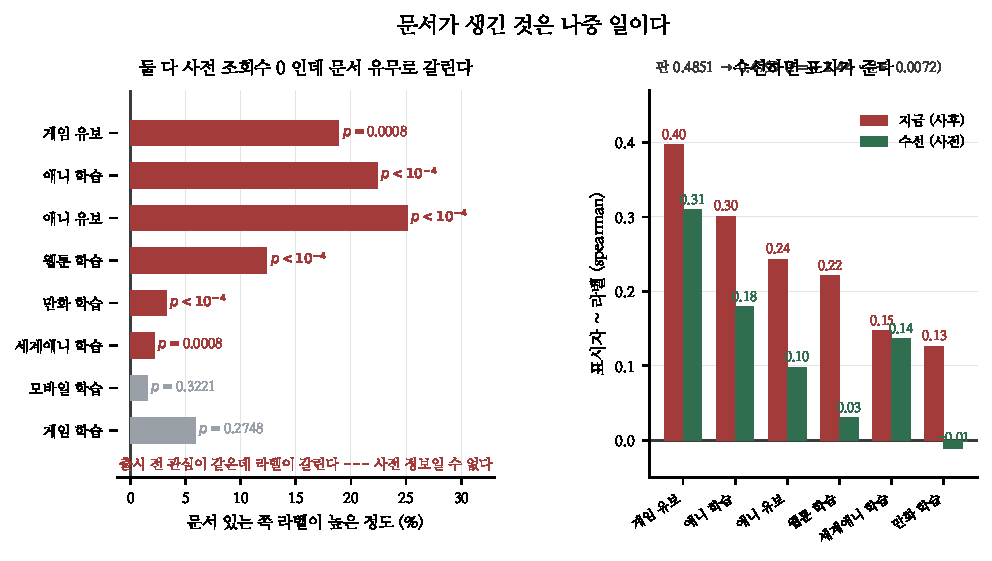
\includegraphics[width=\textwidth]{figs/after.pdf}
\caption{왼쪽 --- 사전 창 조회수가 둘 다 0 인 두 무리의 라벨 차이.
오른쪽 --- 수선 전후의 표시자$\sim$라벨 상관.}
\end{figure*}

\textbf{사전 창 조회수가 둘 다 0} 인데 \textbf{문서 유무만} 다른 두 무리를
견줬다. 둘 다 출시 전 위키 관심이 \emph{정확히 0} 이다.

\begin{center}\footnotesize
\begin{tabular}{llrrrl}
\hline
도메인 & 구간 & 문서없음 & 문서有 & $p$ & \\
\hline
게임 & 유보 & 7.643 & \textbf{9.087} & 0.0008 & $\ast$ \\
애니 & 학습 & 2.049 & 2.508 & $<$1e-4 & $\ast$ \\
애니 & 유보 & 1.663 & 2.081 & $<$1e-4 & $\ast$ \\
웹툰 & 학습 & 4.786 & 5.378 & $<$1e-4 & $\ast$ \\
만화 & 학습 & 3.960 & 4.089 & $<$1e-4 & $\ast$ \\
세계애니 & 학습 & 4.649 & 4.749 & 0.0008 & $\ast$ \\
모바일 & 학습 & 2.710 & 2.752 & 0.322 & \\
게임 & 학습 & 8.179 & 8.659 & 0.275 & \\
\hline
\end{tabular}
\end{center}

\textbf{여덟 칸 중 여섯이 $p{<}0.01$ 이다.} 출시 전 관심이 같은데 라벨이
갈리므로 \textbf{그 차이는 사전 정보일 수 없다.}

\section{수선}

손잡이는 이미 있었다 --- \texttt{zero\_is\_data=False}. 창에 조회수가
있어야 관측으로 치고, 그러려면 \textbf{문서가 출시 전에 존재해야 한다.}
그러면 표시자가 ``출시 전에 문서가 있었다''가 되어 사전이 된다.

\begin{center}\footnotesize
\begin{tabular}{llrr}
\hline
도메인 & 구간 & 지금 & \textbf{수선} \\
\hline
게임 & 유보 & 0.397 & 0.310 \\
애니 & 학습 & 0.301 & 0.179 \\
\textbf{애니} & 유보 & 0.243 & \textbf{0.098} \\
\textbf{웹툰} & 학습 & 0.221 & \textbf{0.030} \\
\textbf{만화} & 학습 & 0.126 & \textbf{$-$0.011} \\
세계애니 & 학습 & 0.147 & 0.136 \\
\hline
\end{tabular}
\end{center}

애니 · 웹툰 · 만화는 사실상 사라진다. \textbf{게임 유보는 0.31 로 남는데
그것은 남아야 하는 것이다} --- 수선 뒤 표시자는 ``출시 전에 문서가 있었고
조회수가 있었다''이고 그건 \textbf{진짜 사전 관심}이다.

\paragraph{대가}

\begin{center}\small
\begin{tabular}{lrrr}
\hline
& 지금 & 수선 & $t$ \\
\hline
\textbf{판} & 0.4851 & \textbf{0.4799} & $-$1.44 \\
게임 & 0.6214 & 0.5893 & $-$2.23 \\
애니 & 0.5012 & 0.4764 & $-$2.27 \\
세계애니 & 0.5336 & 0.5475 & $+$1.79 \\
나머지 일곱 & \multicolumn{3}{c}{$|t|{<}1.1$} \\
\hline
\end{tabular}
\end{center}

판 $\Delta{=}{-}0.0052$ 에 문턱 0.0072 --- \textbf{못 가른다.} 그리고 비용이
\textbf{표지가 있던 두 도메인에서만} 난다. 도메인 문턱($|t|{>}2.77$)을 넘는
것은 없다.

\paragraph{내려가도 되돌리지 않는다} 배포 규칙(노트 275)은 \emph{개선}을
거르는 장치다. 이것은 개선이 아니라 \textbf{정정}이고, 사전 등록에 그렇게
적어 뒀다. \textbf{배포했다} --- \texttt{lab/loop.py} 의 \texttt{\_wiki}
기본값을 바꾸고, 축 정의가 바뀌었으므로 \texttt{denominator.json} 에
새 기준선 \textbf{0.4799} 를 명시적으로 다시 놓았다(노트 284의 규약).
지문도 바뀐다.

\section{검색 축은 왜 괜찮은가}

같은 의심을 검색 계열에 붙여 보면 구조가 다르다.

\begin{center}\footnotesize
\begin{tabular}{ll}
\hline
위키 & 문서가 없으면 \textbf{물어볼 대상이 없다} \\
검색 & 물어보고 \textbf{빈 계열을 받는다} \\
\hline
\end{tabular}
\end{center}

수집기는 데이터랩에 검색어를 물어보고 빈 계열이 오면 그것을 ``아무도 안
찾았다''로 기록한다 --- \textbf{수집 시점의 진짜 측정}이고, 창이 오픈 210일
전부터라 계열이 오기만 하면 오픈 이전 점이 반드시 넷 이상 나온다(노트의
\texttt{\_state} 주석). 검색에서 마스크 0 은 \textbf{그 레코드의 검색어를
아예 모른다}는 뜻이지 결과가 아니다.

\textbf{그래서 이것은 ``모든 표시자가 의심스럽다''가 아니라 위키 하나의
구조적 문제다.}

\paragraph{남은 것}
\begin{center}\small
\begin{tabular}{ll}
\hline
갈래 & 왜 \\
\hline
표시자 감사를 가드로 & 표시자$\sim$라벨을 자동으로 \\
게임 위키 0.31 & 진짜 사전인지 한 번 더 \\
태그 · 달력 표시자 & 달력은 100\% 라 상수 \\
피처 위약 & 노트 302의 갈래 --- 돌고 있다 \\
\hline
\end{tabular}
\end{center}

\paragraph{규약} \textbf{축의 출처를 등록할 때 값과 표시자를 따로 물어라.}
\texttt{provenance} 가 \texttt{wiki\_*} 를 ``시작일 이전 90일''로 PRE 에
올려 뒀고 그 문장은 참이었다 --- \emph{값에 대해서만}. \texttt{forms.\_design}
이 (값, 표시자) 쌍을 내므로 표시자는 별도의 열이고 별도의 출처를 가진다.
그리고 \textbf{다른 것을 재려다 걸린 것을 그냥 지나치지 마라} --- 오늘
덮음을 세려던 표에서 이것이 나왔고, 갈래에 적힌 숫자는 낡아 있었다.

\end{document}
